\section{InstructionAPI Modules and Abstractions}

The Instruction API contains three major components: the top-\/level instruction
representation, the abstract syntax trees representing the operands of an
instruction, and the decoder that creates the entire representation. We will
present an overview of the features and uses of each of these three components,
followed by an example of how the Instruction API can be applied to binary
analysis. 

\subsection{Instruction Interface}

The Instruction API represents a machine language instruction as an Instruction
object, which contains an Operation and a collection of Operands. The Operation
contains the following items:

\begin{itemize}
\item The mnemonic for the machine language instruction represented by its associated Instruction
\item The number of operands accepted by the Operation
\item Which Operands are read and/or written by the associated machine operation
\item What other registers (if any) are affected by the underlying machine operation
\end{itemize}

Each Operand contains flags to indicate whether it is read, written, or both by
the machine instruction represented by its parent Instruction, and contains a
Expression abstract syntax tree representing the operations required to compute
the value of the operand. Figure~\ref{fig:ownership-graph} depicts these
ownership relationships within an Instruction. 

\begin{figure}
\centering
    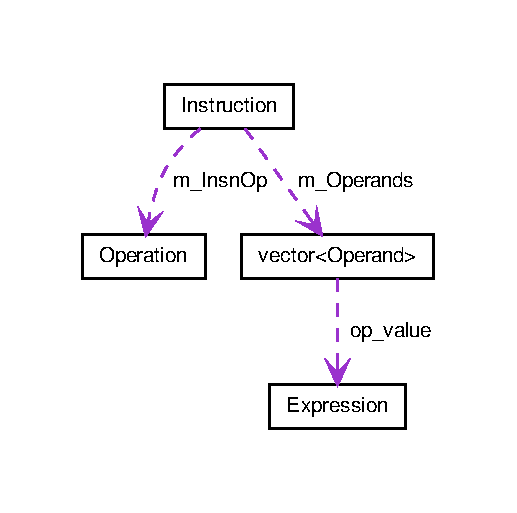
\includegraphics{fig/ownership_graph}
\caption{An Instruction and the objects it owns}
\label{fig:ownership-graph}
\end{figure}

Instruction objects provide two types of interfaces: direct read access to their
components, and common summary operations on those components. The first
interface allows access to the Operation and Operand data members, and each
Operand object in turn allows traversal of its abstract syntax tree. More
details about how to work with this abstract syntax tree can be found in
Section~\ref{subsec:hierarchy}.
This interface would be used, for example, in a data flow analysis where a user wants
to evaluate the results of an effective address computation given a known
register state.

The second interface allows a user to get the sets of registers read and written
by the instruction, information about how the instruction accesses memory, and
information about how the instruction affects control flow, without having to
manipulate the Operands directly. For instance, a user could implement a
register liveness analysis algorithm using just this second interface (namely
the \code{getReadSet} and \code{getWriteSet} functions).

\subsection{Instruction Decoding}

An InstructionDecoder interprets a sequence of bytes according to a given
machine language and transforms them into an instruction representation. It
determines the opcode of the machine instruction, translates that opcode to an
Operation object, uses that Operation to determine how to decode the
instruction's Operands, and produces a decoded Instruction.

\begin{figure}
    \centering
    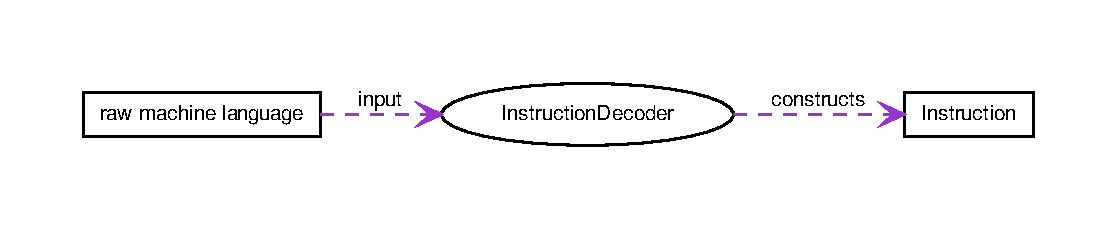
\includegraphics[scale=.8]{fig/decoder_use}
\caption{The InstructionDecoder's inputs and outputs}
\label{fig:decoder-use}
\end{figure}
 
Instruction decoders are built from the following elements:

\begin{itemize}
\item A function to find and extract an opcode given a pointer into a buffer that points to the beginning of a machine instruction
\item A table that, for a particular architecture, maps opcodes to Operations and functions that decode Operands
\end{itemize}

From these elements, it is possible to generalize the construction of
Instructions from Operations and Operands to an entirely platform-\/independent
algorithm. Likewise, much of the construction of the ASTs representing each
operand can be performed in a platform-\/independent manner. 

\subsection{InstructionAST Hierarchy}
\label{subsec:hierarchy}

The AST representation of an operand encapsulates the operations performed on
registers and immediates to produce an operand for the machine language
instruction.

The inheritance hierarchy of the AST classes is shown in
Figure~\ref{fig:inheritance}. 
\begin{figure}
    \centering
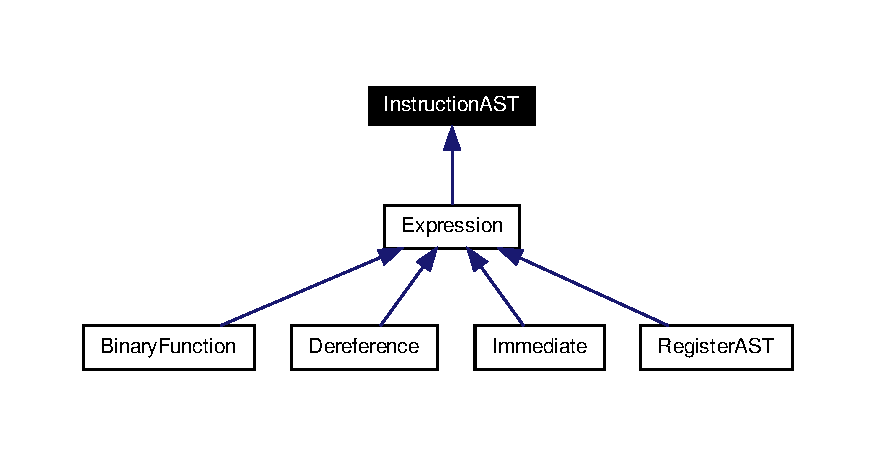
\includegraphics{fig/full_inheritance_graph}
\caption{The InstructionAST inheritance hierarchy}
\label{fig:inheritance}
\end{figure}

The grammar for these AST representations is simple: all leaves must be
RegisterAST or Immediate nodes. These nodes may be combined using a
BinaryFunction node, which may be constructed as either an addition or a
multiplication. Also, a single node may descend from a Dereference node, which
treats its child as a memory address. Figure~\ref{fig:ownership} shows the allowable parent/child
relationships within a given tree, and Figure~\ref{fig:representation} shows how an example IA32
instruction is represented using these objects. 

\begin{figure}
    \centering
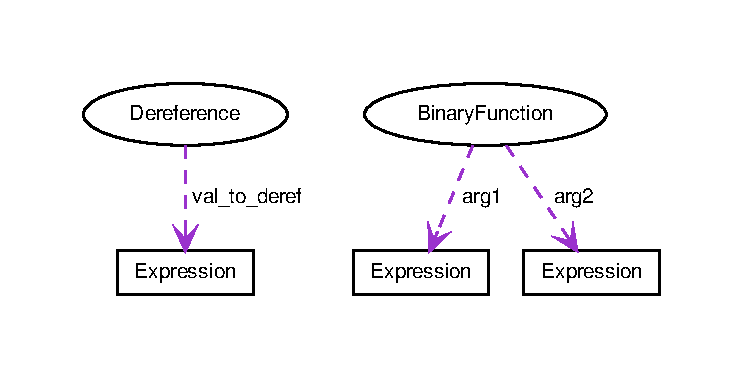
\includegraphics{fig/ast_ownership}
\caption{InstructionAST intermediate node types and the objects they own}
\label{fig:ownership}
\end{figure}
 
\begin{figure}
    \centering
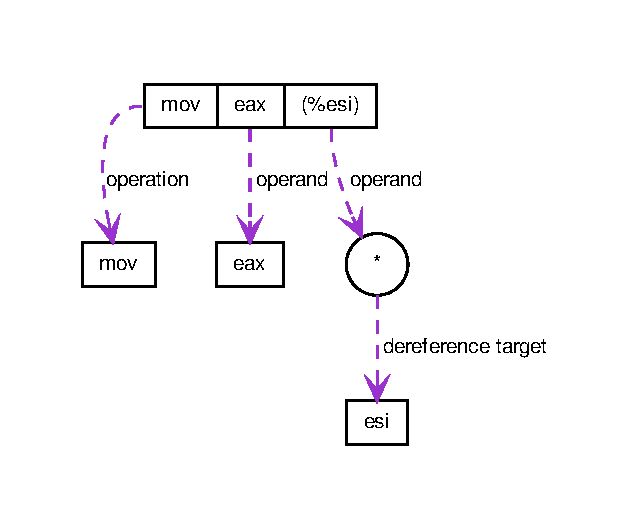
\includegraphics{fig/instruction_representation}
\caption{The decomposition of \code{mov} \code{\%eax}, (\code{\%esi})}
\label{fig:representation}
\end{figure}

These ASTs may be searched for leaf elements or subtrees (via 
\code{getUses} and \code{isUsed}) and traversed breadth-\/first or depth-\/first
(via \code{getChildren}).

Any node in these ASTs may be evaluated. Evaluation attempts to determine the
value represented by a node. If successful, it will return that value and cache
it in the node. The tree structure, combined with the evaluation mechanism,
allows the substitution of known register and memory values into an operand,
regardless of whether those values are known at the time an instruction is
decoded. More details on this mechanism may be found in
Section~\ref{sec:expression}.
